\chapter{Recherche Opérationnel}
\pagebreak

\section{Rappel}
\subsection{Pivot de gauss}

$ L1 et L2 =
\begin{cases}
L1: 160 = 8x + 4y\\
L2: 120 = 4x + 6y 
\end{cases}$
\\
$( L2*(-2) )=
\begin{cases}
L1: 160 = 8x + 4y\\
L2: -240 = -8x -12y
\end{cases}$
\\
$( L2=L2+L1 )=
\begin{cases}
L1: 160 = 8x + 4y\\
L2: -80 = -8y
\end{cases}$
\\
$y = 10$
\\\\
$8x + 4*10 = 160$\\
$8x + 40 = 160$\\
$8x = 120$\\
$x = 15$\\

\section{Introduction à la PL}

Construire une modèle linéaire, c'est donc:
\begin{description}
\item[identifier] les variables de décision du problème
\item[déterminer]: la fonction objectif du modèle
\item[déterminer]: les contraintes du modèle 
\end{description}

\subsection{Modèle linéaire continus à 2 variables}
Soit le modèle linéaire suivantes:
\pagebreak
\begin{description}
\item[Déterminer] $(x,y) \in \Im^2$
\item[Minimisant] $z = 1000x + 1200y$
\item[sous les contraintes]:
\begin{description}
\item[] $(1) 8x + 4y \leq 160$
\item[] $(2) 4x + 6y \leq 120$
\item[] $(3) x \leq 34$
\item[] $(4) y \leq 14$
\item[] $(5) 0 \leq x$
\item[] $(6) 0 \leq y$
\end{description}
\end{description}

\subsubsection{Recherche de solutions}
Après avoir tracé graphiquement tout les points:\\
Pour chaque contrainte, tracer la droite et repérer le demi plan des solution: exemple pour (5) et (6), x et y doivent être supérieurs ou égal à 0, d'où le demi plan des solution sont toutes les valeurs positives.\\
La partie En vert représente la région admissible, quelque soit le point choisis dans ce vert, aucune contrainte ne sera violé.\\
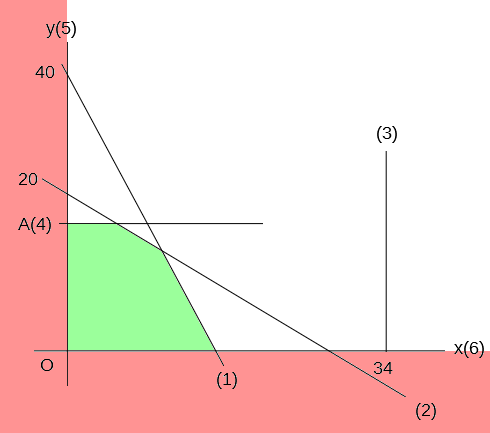
\includegraphics[scale=0.55]{img/ro-pl-2var_0.png} 
\subsubsection{recherche de la solution optimal}

Changer l'équation $z$ tel que $z$ soit égal à $0$
\begin{description}
\item[$z$] = $1000x + 1200y$ = $0$ = $1000*(1200) + 1200 *(-1000)$
\end{description}
Traçons la droite $(0,0)$, $(1200,-1000)$
\begin{description}
\item[Un point extrême]: est un point se trouvant sur l'intersection de 2 contraintes et étant dans la zone admissible.
\item[L'altitude]: est la droite (rouge) la plus haute touchant un point extrême, ce point sera le vecteur $(x,y)$ le plus optimal pour $z$.
\item[] Les droites rouges doivent être toutes parallèles.
\end{description}
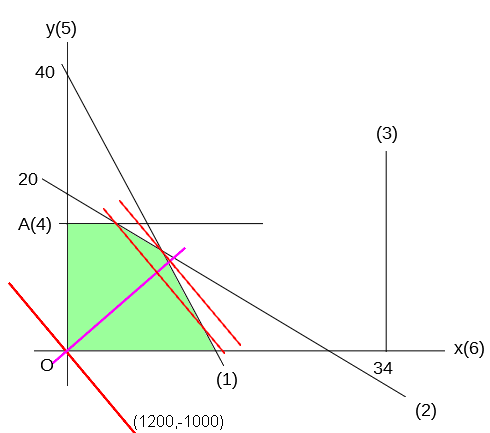
\includegraphics[scale=0.55]{img/ro-pl-2var_1.png} \\
Dans cette exemple le point (15,10) est le point extrême maximal pour l'équation z.\\

\pagebreak